%=====================================================================
%  IEEE i-COSTE 2026 -- camera-ready version (Paper ID: ieee-icoste_3738)
%  Confidence-Aware RAG with Abstention for Cyber Threat Intelligence
%
%  Format: IEEE two-column conference, max 6 pages incl. authors and refs.
%  Compile from the repository root so figures/ resolves:
%      pdflatex icoste2026_camera ; pdflatex icoste2026_camera
%
%  All numbers are taken from results/*.csv (the 200-query main run).
%  Fig. 2 is produced by plot_risk_coverage.py from the same files.
%=====================================================================
\documentclass[conference]{IEEEtran}
\IEEEoverridecommandlockouts

\usepackage{cite}
\usepackage{amsmath,amssymb,amsfonts}
\usepackage{graphicx}
\usepackage{booktabs}
\usepackage{array}
\usepackage{tabularx}
\usepackage{multirow}
\usepackage{xcolor}
\usepackage{url}
\usepackage{algorithm}
\usepackage{algorithmic}
\usepackage[T1]{fontenc}
\usepackage{enumitem}
\usepackage{microtype}
\usepackage[hidelinks]{hyperref}  % clickable citations and cross-references

\begin{document}

\title{Confidence-Aware Retrieval-Augmented Generation\\ with Abstention for Cyber Threat Intelligence}

\author{%
\IEEEauthorblockN{1\textsuperscript{st} Md.~Latifur Rahman Rafi}
\IEEEauthorblockA{\textit{Dept. of Computer Science and Engineering} \\
\textit{Daffodil International University} \\
Dhaka, Bangladesh \\ latifur23105101451@diu.edu.bd}
\and
\IEEEauthorblockN{2\textsuperscript{nd} Fernaz Narin Nur}
\IEEEauthorblockA{\textit{Dept. of Computer Science and Engineering} \\
\textit{Daffodil International University} \\
Dhaka, Bangladesh \\ fernaznur@gmail.com}
\and
\IEEEauthorblockN{3\textsuperscript{rd} Md.~Minhajul Islam}
\IEEEauthorblockA{\textit{Dept. of Computer Science and Engineering} \\
\textit{Daffodil International University} \\
Dhaka, Bangladesh \\ islam2305101257@diu.edu.bd}
\and
\IEEEauthorblockN{4\textsuperscript{th} Md.~Hasanuzzaman Dipu}
\IEEEauthorblockA{\textit{Dept. of Computer Science and Engineering} \\
\textit{Daffodil International University} \\
Dhaka, Bangladesh \\ hdipu2646@gmail.com}
\and
\IEEEauthorblockN{5\textsuperscript{th} Nazmun Nessa Moon}
\IEEEauthorblockA{\textit{Dept. of Computer Science and Engineering} \\
\textit{Daffodil International University} \\
Dhaka, Bangladesh \\ moon@daffodilvarsity.edu.bd}
\and
\IEEEauthorblockN{6\textsuperscript{th} A.~H.~M.~Saiful Islam}
% CHECK: the e-mail domain ndub.edu.bd is Notre Dame University Bangladesh;
% confirm this author's affiliation before submission.
\IEEEauthorblockA{\textit{Dept. of Computer Science and Engineering} \\
\textit{Daffodil International University} \\
Dhaka, Bangladesh \\ saiful@ndub.edu.bd}
}

\maketitle

%====
\begin{abstract}
Retrieval-Augmented Generation (RAG) grounds language models in external
knowledge, which makes it a natural tool for Cyber Threat Intelligence
(CTI). Standard RAG, however, answers every question, even when the
retrieved evidence does not support an answer, and can mislead an analyst
with invented vulnerability details. We study a confidence-aware RAG
pipeline for CVE search that declines to answer when a retrieval-stage
confidence score falls below a threshold. The score combines the
similarity of the best-matching record with its margin over the second
record, and needs no access to the language model's internals. On 200
automatically generated keyword queries over the 2023 National
Vulnerability Database (30{,}932 CVE records), the gate abstains on 16\%
of queries and raises precision on answered queries to 75.6\%, against
70.0\% for BM25-only RAG and 73.7\% for the same hybrid pipeline without
the gate. The rejected queries are genuinely hard: the ungated system
answers only 31.3\% of them correctly. Raising the threshold trades
coverage for precision, up to 85.0\% at 20\% coverage. We also show that
the score ranks answers by reliability (AUROC 0.70) but is not a
calibrated probability, and we explain why Expected Calibration Error
favours the ungated baseline.
\end{abstract}

\begin{IEEEkeywords}
Retrieval-Augmented Generation, Cyber Threat Intelligence, confidence
estimation, abstention, selective prediction, CVE, NVD.
\end{IEEEkeywords}

%=====================================================================
\section{Introduction}
%=====================================================================
Cyber Threat Intelligence (CTI) analysts spend much of their day searching
large vulnerability databases, such as the National Vulnerability Database
(NVD)~\cite{ref_wagner}, for precise information. In this setting a wrong
answer is expensive. A single incorrect CVE reference can lead an analyst
to patch the wrong software, miss a real exposure, or misdirect an
incident response. A system that answers confidently but incorrectly is
therefore more harmful than one that admits it does not know.

Retrieval-Augmented Generation (RAG)~\cite{ref_lewis} is a natural fit for
this task. It retrieves relevant documents and lets a language model write
an answer grounded in them. Standard RAG pipelines never check whether the
retrieved evidence actually supports the question. When retrieval fails,
the model still produces a fluent but wrong answer. This is especially
harmful in CVE-based CTI, where severity scores, affected versions, and
weakness categories must be exact.

Most ways of estimating confidence do not fit this setting. Some read the
model's token probabilities~\cite{ref_varshney}, which small, locally
hosted models often do not expose. Others measure uncertainty only in the
generated text~\cite{ref_kuhn} and ignore the retrieval stage, where the
uncertainty in CVE search begins. Methods that act at retrieval time, such
as REPLUG~\cite{ref_replug}, reweight documents but give no signal for
deciding when the evidence is too weak to answer at all.

\noindent\textit{Contributions:} This paper makes four contributions.
\begin{itemize}[leftmargin=1.4em,topsep=2pt,itemsep=2pt]
\item A retrieval-only abstention gate for CTI question answering. It
decides before generation, so rejected queries cost no language-model
call and need no model internals.
\item An analysis of which retrieval signal carries the information. In
hybrid retrieval the most useful signal is agreement between the lexical
and dense retrievers, while the margin term adds little.
\item A precision-coverage study over the full query set, with paired
significance tests, bootstrap confidence intervals, and a quantitative
analysis of over-abstention and over-confident errors.
\item A careful treatment of calibration for generative retrieval. We
define how Expected Calibration Error (ECE) is computed with abstention and
show why it can reward an uninformative baseline.
\end{itemize}

The rest of this paper is organized as follows.
Section~\ref{sec:related} reviews related work. Section~\ref{sec:method}
presents the framework. Section~\ref{sec:setup} describes the experimental
setup. Section~\ref{sec:results} reports the results.
Section~\ref{sec:discussion} discusses failure modes and generalizability,
and Section~\ref{sec:conclusion} concludes the paper.

%=====================================================================
\section{Related Work}
\label{sec:related}
%=====================================================================
Table~\ref{tab:litreview} groups the most relevant prior work and shows
where our system fits.

\begin{table*}[t]
\caption{Representative related work and positioning of our approach.}
\label{tab:litreview}
\centering
\footnotesize
\setlength{\tabcolsep}{5pt}
\renewcommand{\arraystretch}{1.12}
\begin{tabularx}{\textwidth}{@{}l l l X X@{}}
\toprule
Ref & Study & Yr & Approach / contribution & Limitation we address \\
\midrule
\cite{ref_lewis} & Lewis et al. & 2020 & DPR\,+\,BART RAG; retrieval and generation integration & Fixed top-$K$; no confidence signal \\
\cite{ref_selfrag} & Asai et al. & 2024 & Self-RAG: adaptive retrieval with reflection tokens & Requires a fine-tuned generator \\
\cite{ref_crag} & Yan et al. & 2024 & CRAG: retrieval evaluator triggers correction and web search & Corrects rather than abstains \\
\cite{ref_replug} & Shi et al. & 2024 & REPLUG: black-box reweighting by similarity & No abstention decision \\
\cite{ref_qpp} & Cronen-Townsend et al. & 2002 & Query performance prediction from retrieval scores & Not used to gate generation \\
\cite{ref_selective}, \cite{ref_kamath} & Geifman; Kamath et al. & 2017; 2020 & Selective prediction and selective QA with risk-coverage analysis & Not studied for CTI retrieval \\
\cite{ref_calibration} & Guo et al. & 2017 & Expected Calibration Error (ECE) & Defined for classification only \\
\cite{ref_cybermetric} & Tihanyi et al. & 2024 & CyberMetric: cybersecurity LLM benchmark & Closed-book; no retrieval gate \\
\midrule
\multicolumn{2}{@{}l}{This work} & 2026 & Retrieval-only abstention gate for NVD search; precision-coverage study & Keyword queries; single corpus \\
\bottomrule
\end{tabularx}
\end{table*}

\noindent\textit{RAG and adaptive retrieval:} The original RAG
framework~\cite{ref_lewis} always retrieves a fixed number of documents.
Self-RAG~\cite{ref_selfrag} learns when to retrieve and critiques its own
output, but it needs a specially trained generator. CRAG~\cite{ref_crag}
scores retrieval quality with a trained evaluator and, when it is low,
corrects the context with web search instead of abstaining.
REPLUG~\cite{ref_replug} reweights documents for a frozen model but never
declines to answer.

\noindent\textit{Retrieval confidence and selective prediction:} Using
retrieval scores to predict whether a search will succeed is an old idea
in information retrieval, known as query performance
prediction~\cite{ref_qpp}. Abstaining when confidence is low is studied as
selective prediction~\cite{ref_selective} and, for question answering, as
selective QA~\cite{ref_kamath}; both evaluate with risk-coverage curves,
which we adopt. Our score is a simple member of this family, so we do not
claim a new uncertainty estimator. Our contribution is to use such a score
as a pre-generation gate for CTI with a local model, to identify which
signal drives it in hybrid retrieval, and to evaluate the resulting
trade-off reproducibly. Dense retrievers~\cite{ref_dpr} and
BM25~\cite{ref_bm25} are complementary, and reciprocal rank
fusion~\cite{ref_rrf} is a standard way to combine them~\cite{ref_hhr}.
Semantic entropy~\cite{ref_kuhn} and self-evaluation~\cite{ref_kadavath}
estimate uncertainty from the generator instead, and
CySecBERT~\cite{ref_cysecbert} adapts encoders to security text. CTI
surveys flag relevance filtering as an open problem~\cite{ref_wagner}.

%=====================================================================
\section{Proposed Framework}
\label{sec:method}
%=====================================================================
\begin{figure*}[t]
\centering
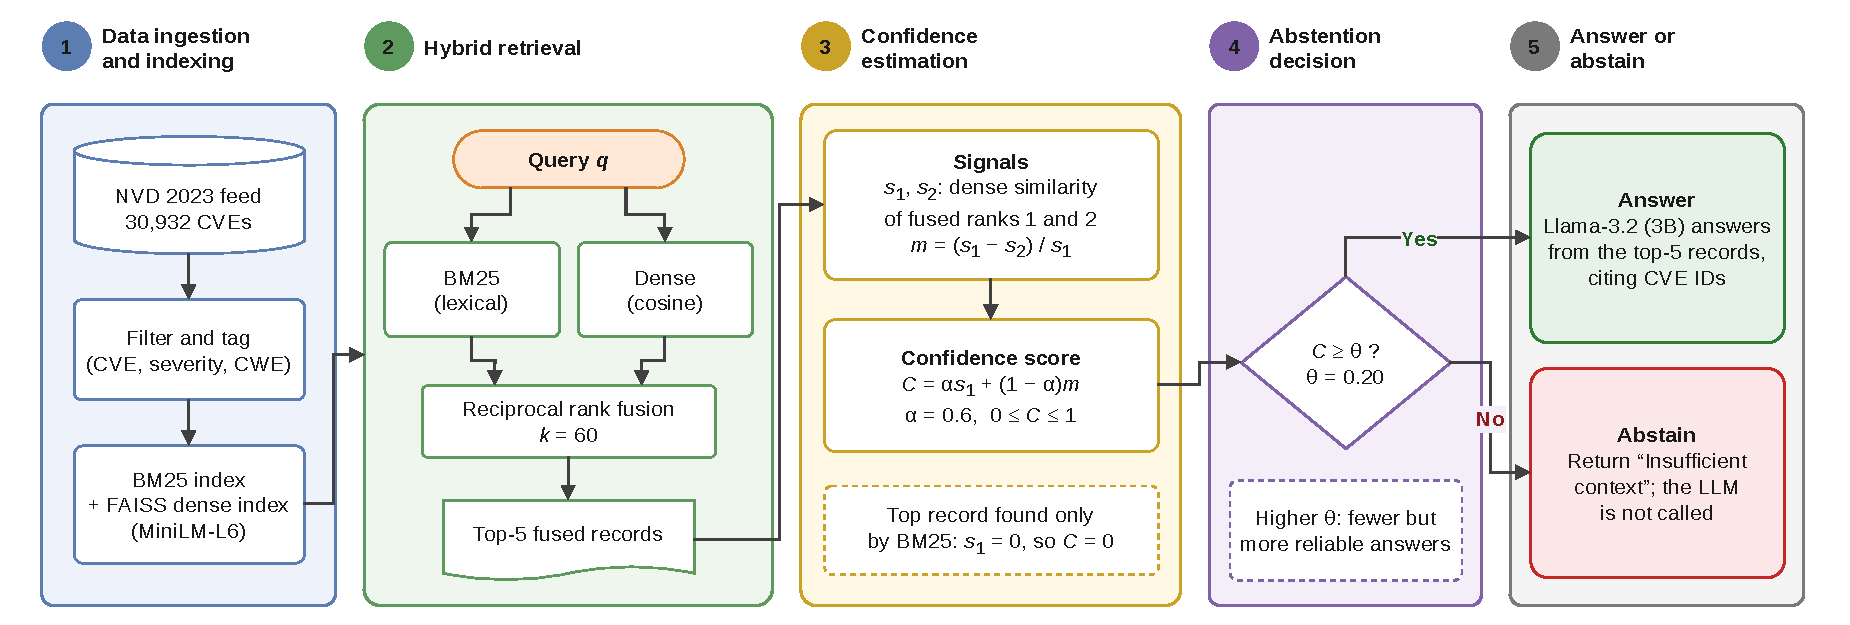
\includegraphics[width=\textwidth]{figures/fig1_pipeline.pdf}
\caption{Overview of the Confidence-Aware RAG pipeline. Hybrid BM25,
dense, and reciprocal-rank-fusion retrieval feed a retrieval-stage
confidence score $C$. A threshold $\theta$ then decides between answering
and abstaining.}
\label{fig:methodology}
\end{figure*}

Fig.~\ref{fig:methodology} gives an overview. A query passes through
hybrid retrieval, a confidence score is computed from the retrieval
scores, and a threshold decides whether the system answers or abstains.

\subsection{Dataset}
Our knowledge base is the 2023 NVD JSON feed (version 2.0). We drop
records whose description is shorter than 50 characters, which leaves
30{,}932 entries. Each record carries a CVE identifier, a CVSS severity, a
CWE category, and a free-text description. Before indexing, we prepend a
short tag with the CVE identifier, severity, and CWE code to each
description, which helps BM25 match exact identifiers.

\subsection{Problem Formulation}
Given a query and the corpus, retrieval returns the top-$K$ records, a
confidence step scores the retrieval with a value $C\in[0,1]$, and a
generator writes an answer from the records. A threshold $\theta$ controls
the system:
\begin{equation}
\text{decision}=
\begin{cases}
\text{answer}, & C \ge \theta,\\[2pt]
\text{abstain}, & C < \theta.
\end{cases}
\label{eq:gate}
\end{equation}
When the system abstains, it returns an ``Insufficient context'' message
and does not call the language model.

\subsection{Hybrid Retrieval}
\noindent\textit{Sparse retrieval:} A BM25 index~\cite{ref_bm25} over the
tagged descriptions recalls exact identifiers, CWE codes, and product
names. Tokenisation strips punctuation but keeps hyphens.

\noindent\textit{Dense retrieval:} We encode every record with
all-MiniLM-L6-v2~\cite{ref_sbert} and search the normalised
384-dimensional vectors exactly with FAISS (inner product, equal to cosine
similarity).

\noindent\textit{Reciprocal rank fusion:} Each retriever returns $2K$
candidates, which we merge with reciprocal rank fusion~\cite{ref_rrf}:
\begin{equation}
\mathrm{RRF}(d)=\!\!\sum_{r\in\{r_{\mathrm{BM25}},\,r_{\mathrm{dense}}\}}\!\!
\frac{1}{k+\mathrm{rank}_r(d)},\quad k=60.
\label{eq:rrf}
\end{equation}
The constant $k=60$ is the value recommended in~\cite{ref_rrf}. The top
$K=5$ fused records go to the confidence step.

\subsection{Confidence Scoring}
Let $s_1$ and $s_2$ be the dense cosine similarities of the first and
second fused records. The confidence score is
\begin{equation}
C=\alpha\, s_1+(1-\alpha)\,m,\qquad
m=\frac{s_1-s_2}{s_1},\quad \alpha=0.6.
\label{eq:conf}
\end{equation}
The first term reflects raw match quality. The margin $m$ reflects how
clearly the top record stands out; a near tie suggests an ambiguous query.
A record that only BM25 retrieved has no dense similarity and is assigned
a similarity of zero. When such a record is ranked first, $C=0$. This case
means the two retrievers disagree about the best record, and it turns out
to be the strongest signal in our data (Section~\ref{sec:results}).

\noindent\textit{Parameter choice:} We fixed $\alpha=0.6$ and
$\theta=0.20$ during development on the same query distribution; there
was no separate validation split. We therefore report sensitivity to both
parameters in Section~\ref{sec:results} rather than presenting them as
tuned optima.

\subsection{Answer Generation}
When the gate allows an answer, the five top records are passed to
Llama-3.2 (3B), run locally through Ollama~\cite{ref_llama}, with greedy
decoding and a 512-token limit. The prompt tells the model to use only the
supplied records, to say so when they are insufficient, and to cover the
vulnerability, affected component, severity, and impact. Algorithm
\ref{alg:conf_rag} summarises the pipeline.

\begin{algorithm}[t]
\caption{Confidence-Aware RAG with Abstention}
\label{alg:conf_rag}
\small
\begin{algorithmic}[1]
\REQUIRE query $q$, corpus $\mathcal{C}$, threshold $\theta$, top-$K$,
weight $\alpha$
\ENSURE answer $a$ or an abstention signal
\STATE $R_{\mathrm{BM25}}\leftarrow\text{BM25}(q,\mathcal{C},2K)$
\STATE $R_{\mathrm{dense}}\leftarrow\text{DenseSearch}(q,\mathcal{C},2K)$
\STATE $R\leftarrow\text{RRF}(R_{\mathrm{BM25}},R_{\mathrm{dense}},k{=}60)[{:}K]$
\STATE get dense similarities $s_1,s_2$ of the top two records in $R$
\STATE $m\leftarrow(s_1-s_2)/s_1$;\ \ $C\leftarrow\alpha s_1+(1-\alpha)m$
\IF{$C\ge\theta$}
    \STATE $a\leftarrow\text{LLM}(q,R,\text{temp}{=}0,\text{max\_tok}{=}512)$
    \RETURN $a$ with source citation
\ELSE
    \RETURN ``Insufficient context''
\ENDIF
\end{algorithmic}
\end{algorithm}

\noindent\textit{Worked example:} For the query ``Apache HTTP/2 rapid
reset denial of service'', both retrievers agree on CVE-2023-44487, and
$C=0.36$, so the system answers. The vague query ``recent Linux bug''
gives two records with identical similarity (0.54), so the margin is zero
and $C=0.33$; the system answers at $\theta=0.20$ but would abstain at
$\theta\ge0.35$. For ``Incorrect X-Forwarded-For pretix Incorrect
parsing'', BM25 ranks the correct record first but the dense retriever
does not return it, so $C=0$ and the system abstains even though the
answer was available. Section~\ref{sec:discussion} analyses such cases.

%=====================================================================
\section{Experimental Setup}
\label{sec:setup}
%=====================================================================
\noindent\textit{Queries and gold answers:} We sample 200 CVE records
uniformly at random (seed 42). For each record, a query of up to five
keywords is extracted automatically from its description with one of three
templates: technical terms (51.5\% of queries), severity plus
vulnerability type (28.5\%), and product names (20.0\%). CVE identifiers
are removed from the query. Examples are ``Linux kernel rose\_ioctl'' and
``MEDIUM Scripting Cross-Site Scripting 3.1.6 Auth''. This is a
known-item setting: each query has one target record, whose NVD
description serves as the gold answer. The queries are not written by
analysts, and because they reuse words from the target record they favour
lexical retrieval. The results therefore measure confidence-based
selective answering in a controlled, reproducible CTI retrieval setting,
not performance on unrestricted analyst queries
(Section~\ref{sec:discussion}).

\noindent\textit{Systems compared:} Naive RAG uses BM25 only and never
abstains. Hybrid RAG adds dense search and fusion and never abstains.
Confidence-Aware RAG is Hybrid RAG with the gate at $\theta=0.20$. All
three use the same generator and prompt. The language model may still
refuse on its own; Hybrid RAG did so for 14 queries.

\noindent\textit{Evaluation metrics:} We group the metrics by what they
measure. Retrieval is measured by Recall@5, the share of queries whose
target record is in the top five. Answer quality is ROUGE-L F1 against the
gold description, over all queries (abstentions score zero) and over
answered queries. An answer counts as correct when its ROUGE-L is at least
0.20, and reliability is Precision@Answered, the share of answered queries
that are correct. Coverage is the share of queries answered.

\noindent\textit{Confidence quality:} We report two measures, both using
the correctness label above. Discrimination is the AUROC of $C$ for
separating correct from incorrect answers. Calibration is ECE with ten
equal-width bins on $[0,1]$~\cite{ref_calibration}:
$\mathrm{ECE}=\sum_{b}\frac{|B_b|}{n}\,\lvert\mathrm{acc}(B_b)-\mathrm{conf}(B_b)\rvert$,
where $\mathrm{acc}$ is the share of correct answers in bin $B_b$ and
$\mathrm{conf}$ its mean confidence. In Table~\ref{tab:main} ECE is taken
over all 200 queries, and an abstained query keeps its confidence and
counts as incorrect. Naive RAG has no dense retriever, so the same formula
is applied with BM25 scores divided by the top BM25 score.

\noindent\textit{Statistics and implementation:} ROUGE-L differences are
tested with paired $t$-tests on per-query scores; with $n=200$ the mean
difference is approximately normal, and we confirm each result with a
Wilcoxon signed-rank test. Precision compares different subsets of
queries, so we use a paired bootstrap with 10{,}000 resamples. All
experiments run on an Apple MacBook Air (M-series, 16\,GB RAM) with fixed
seeds. The gate does not change the answer to an accepted query, so
each threshold in Section~\ref{sec:results} is evaluated by gating the
saved Hybrid RAG answers.

%=====================================================================
\section{Results and Analysis}
\label{sec:results}
%=====================================================================
\subsection{System Comparison}
Table~\ref{tab:main} groups the results by retrieval, answer quality,
reliability, and confidence quality.

\begin{table}[t]
\caption{Results on 200 queries at $\theta=0.20$ (C is the proposed
system). R-L: ROUGE-L over all
queries and over answered queries. Prec: Precision@Answered. Cov: coverage.}
\label{tab:main}
\centering
\footnotesize
\setlength{\tabcolsep}{2.4pt}
\renewcommand{\arraystretch}{1.15}
\begin{tabular}{@{}l c cc cc cc@{}}
\toprule
 & Retr. & \multicolumn{2}{c}{Answer quality} & \multicolumn{2}{c}{Reliability} & \multicolumn{2}{c}{Confidence} \\
\cmidrule(lr){2-2}\cmidrule(lr){3-4}\cmidrule(lr){5-6}\cmidrule(l){7-8}
System & R@5 & R-L & R-L(ans) & Prec & Cov & ECE & AUROC \\
\midrule
A. Naive RAG         & 0.810 & 0.330 & 0.330 & 0.700 & 100\% & 0.038 & 0.690 \\
B. Hybrid RAG        & 0.795 & 0.298 & 0.321 & 0.737 & 93\%  & 0.309 & 0.700 \\
C. Conf-Aware        & 0.795 & 0.280 & 0.334 & 0.756 & 84\%  & 0.259 & 0.700 \\
\bottomrule
\end{tabular}
\end{table}

\noindent\textit{Retrieval and answer quality:} BM25 alone gives the
highest Recall@5 (0.810), as expected for keyword queries built from the
target record. The gate does not change retrieval. Over all queries
Confidence-Aware RAG has lower ROUGE-L than Naive RAG, because each
abstention scores zero (mean difference $-0.050$, $t(199)=-5.12$,
$p<0.001$, $d_z=-0.36$, 95\% CI $[-0.068,-0.031]$). On the 168 queries it
answers, its ROUGE-L does not differ significantly from Naive RAG's
answers to the same queries ($-0.014$, $t(167)=-1.75$, $p=0.08$; Wilcoxon
$p=0.58$).

\noindent\textit{Reliability and coverage:} Confidence-Aware RAG answers
84\% of queries with 75.6\% precision, against 70.0\% for Naive RAG and
73.7\% for Hybrid RAG. The 5.6-point gain over Naive RAG is suggestive
but not significant at this sample size (paired bootstrap 95\% CI
$[-0.8,12.2]$). The clearer evidence is what the gate removes. On the 32
rejected queries, the ungated Hybrid RAG is correct only 31.3\% of the
time, against 75.6\% on the accepted ones (Fisher's exact test, odds ratio
6.8, $p<10^{-5}$). All 14 queries on which the generator refused by itself
also have $C=0$, so the gate catches them before any model call.

\noindent\textit{Calibration:} Naive RAG has by far the lowest ECE (0.038),
but this does not mean it is better calibrated in a useful sense. Its
score lies between 0.60 and 0.94 for every query (mean 0.67), close to its
overall accuracy (0.70), so a nearly constant score matches the average
accuracy. ECE rewards this, yet the score barely separates right from
wrong answers (AUROC 0.69). Our score has a mean of 0.38 against an
accuracy near 0.70, so it is not a calibrated probability, which explains
its high ECE. Most of the drop from 0.309 to 0.259 between Hybrid and
Confidence-Aware RAG comes from the abstained queries (score 0, counted
incorrect); on answered queries alone ECE is 0.333 and 0.309. We
therefore treat $C$ as a ranking signal for selective answering, and
AUROC and precision-coverage, rather than ECE, as the relevant measures.

\subsection{Ablation of the Confidence Score}
Table~\ref{tab:ablation} compares the full score with each term alone,
ranking all 200 queries and answering the top 84\% or 50\%.

\begin{table}[t]
\caption{Ablation of the confidence score (200 queries). Precision@Answered
at matched coverage.}
\label{tab:ablation}
\centering
\footnotesize
\setlength{\tabcolsep}{4pt}
\renewcommand{\arraystretch}{1.15}
\begin{tabular}{@{}l ccc@{}}
\toprule
Score variant & AUROC & Prec @ 84\% cov. & Prec @ 50\% cov. \\
\midrule
Full, $\alpha=0.6$ (ours)     & 0.700 & 0.756 & 0.780 \\
Similarity only, $\alpha=1$   & 0.699 & 0.756 & 0.810 \\
Margin only, $\alpha=0$       & 0.637 & 0.708 & 0.770 \\
No gate (Hybrid RAG)          & n/a   & \multicolumn{2}{c}{0.737 at 93\% cov.} \\
\bottomrule
\end{tabular}
\end{table}

The top-1 similarity carries almost all of the signal; the margin alone is
clearly weaker, and adding it to the similarity does not help. At 84\%
coverage the full and similarity-only scores make identical decisions,
because both reject exactly the 32 queries with $C=0$. Varying $\alpha$
from 0.5 to 1.0 changes AUROC only between 0.69 and 0.72, so the choice of
$\alpha$ is not critical.

\subsection{Threshold Sensitivity}
Table~\ref{tab:threshold} and Fig.~\ref{fig:sweep} vary the threshold on
all 200 queries. Every threshold up to 0.22 gives the same decisions as
0.20, because the smallest non-zero score is 0.23. Above that, precision
rises steadily as coverage falls, from 75.6\% at 84\% coverage to 85.0\%
at 20\% coverage. No single threshold is best: 0.20 suits a first-pass
filter, while higher values suit settings where an analyst prefers fewer
but more reliable answers. With 200 queries and no held-out split, these
values should be re-checked on the target query distribution.

\begin{table}[t]
\caption{Threshold sensitivity on 200 queries.}
\label{tab:threshold}
\centering
\footnotesize
\setlength{\tabcolsep}{5pt}
\renewcommand{\arraystretch}{1.15}
\begin{tabular}{@{}c cccc@{}}
\toprule
$\theta$ & Coverage & Answered & Prec@Answered & R-L(ans) \\
\midrule
none & 93.0\% & 186 & 0.737 & 0.321 \\
0.20 & 84.0\% & 168 & 0.756 & 0.334 \\
0.30 & 75.0\% & 150 & 0.780 & 0.340 \\
0.40 & 42.5\% & 85  & 0.800 & 0.363 \\
0.50 & 20.0\% & 40  & 0.850 & 0.385 \\
\bottomrule
\end{tabular}
\end{table}

\begin{figure}[t]
\centering
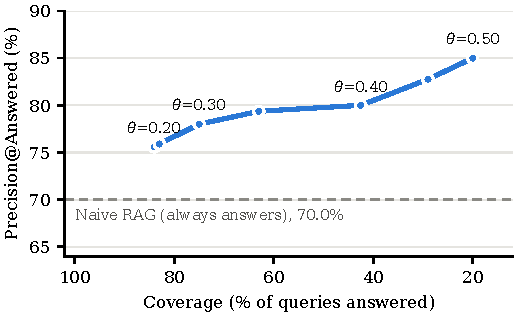
\includegraphics[width=\columnwidth]{figures/fig_risk_coverage.pdf}
\caption{Precision on answered queries against coverage as the threshold
$\theta$ rises (200 queries). The dashed line is Naive RAG, which always
answers.}
\label{fig:sweep}
\end{figure}

%=====================================================================
\section{Discussion}
\label{sec:discussion}
%=====================================================================
\noindent\textit{Over-abstention:} Of the 32 rejected queries, 10 would
have been answered correctly, and for 16 the target record was in the top
five. In these cases BM25 finds the record but the dense retriever does
not, as in the pretix example of Section~\ref{sec:method}. Rejections are
spread evenly over the three query types (11, 11, and 10). Many rejected
queries are strings of version numbers, such as ``14.5 14.6 14.7 HTTP
CVSS'', where abstaining is reasonable.

\noindent\textit{Over-confident errors:} Of the 41 incorrect answers, the
target record was missing from the top five in only 9. Among the 40
answers with $C\ge0.5$, 6 are counted incorrect, and in all 6 the target
was retrieved. For ``Linux kernel rose\_ioctl'' ($C=0.82$) the answer
correctly names CVE-2023-51782 and describes the use-after-free, but its
ROUGE-L is 0.07 because it is formatted as a list. Many such errors thus
reflect the metric rather than the system: a lexical match against the
full NVD description penalises correct answers with different wording.
Product queries are the hardest (46.7\% precision against 79.3\% and
87.0\% for the other types).

\noindent\textit{Generalizability:} Three features of the setup limit how
far the numbers transfer. The keyword queries share words with their
target, which favours BM25 and inflates recall compared with questions
written by analysts. NVD records are short and uniform, whereas real CTI
work mixes advisories, threat reports, and exploit data of varied length
and quality, where retrieval scores behave differently. The gold answers
are lexical, so correctness is measured imperfectly. The qualitative
finding, that a retrieval-only score can separate reliable from
unreliable answers before generation, is likely to hold more broadly, but
the thresholds and the size of the gain must be re-measured on each
deployment's data. A direct comparison with Self-RAG and CRAG on the same
corpus, model, and prompts is also left for future work.

%=====================================================================
\section{Conclusion}
\label{sec:conclusion}
%=====================================================================
We studied a confidence-aware RAG pipeline for CVE search that abstains
when a retrieval-stage score is low. On 200 queries over 30{,}932 NVD
records, the gate removes queries that the ungated system mostly gets
wrong, raises precision on answered queries from 73.7\% to 75.6\% at
84\% coverage, and reaches 85.0\% at 20\% coverage. The score works as a
ranking signal, not a calibrated probability, and its strongest component
is agreement between the lexical and dense retrievers. Future work will
use natural-language analyst queries with a held-out split, factual rather
than lexical answer evaluation, heterogeneous CTI sources, and direct
comparison with generator-side methods. Code, queries, and per-query
results are available at \url{https://github.com/latifurrafi/CTI-RAG}.

%=====================================================================
\begin{thebibliography}{99}
\bibitem{ref_lewis} P.~Lewis \textit{et al.}, ``Retrieval-augmented
generation for knowledge-intensive NLP tasks,'' in \textit{Adv. Neural
Inf. Process. Syst. (NeurIPS)}, vol.~33, 2020, pp.~9459--9474.

\bibitem{ref_selfrag} A.~Asai, Z.~Wu, Y.~Wang, A.~Sil, and
H.~Hajishirzi, ``Self-RAG: Learning to retrieve, generate, and critique
through self-reflection,'' in \textit{Proc. Int. Conf. Learn. Represent.
(ICLR)}, 2024.

\bibitem{ref_crag} S.-Q.~Yan, J.-C.~Gu, Y.~Zhu, and Z.-H.~Ling,
``Corrective retrieval augmented generation,'' \textit{arXiv:2401.15884},
2024.

\bibitem{ref_replug} W.~Shi \textit{et al.}, ``REPLUG:
Retrieval-augmented black-box language models,'' in \textit{Proc. NAACL-HLT},
2024, pp.~8371--8384.

\bibitem{ref_dpr} V.~Karpukhin \textit{et al.}, ``Dense passage
retrieval for open-domain question answering,'' in \textit{Proc. EMNLP},
2020, pp.~6769--6781.

\bibitem{ref_bm25} S.~Robertson and H.~Zaragoza, \textit{The
Probabilistic Relevance Framework: BM25 and Beyond}. Now Publishers,
2009.

\bibitem{ref_rrf} G.~V.~Cormack, C.~L.~A.~Clarke, and S.~Buettcher,
``Reciprocal rank fusion outperforms Condorcet and individual rank
learning methods,'' in \textit{Proc. ACM SIGIR}, 2009, pp.~758--759.

\bibitem{ref_hhr} M.~G.~Arivazhagan \textit{et al.}, ``Hybrid
hierarchical retrieval for open-domain question answering,'' in
\textit{Findings ACL}, 2023, pp.~10680--10689.

\bibitem{ref_sbert} N.~Reimers and I.~Gurevych, ``Sentence-BERT:
Sentence embeddings using Siamese BERT-networks,'' in \textit{Proc.
EMNLP-IJCNLP}, 2019, pp.~3982--3992.

\bibitem{ref_qpp} S.~Cronen-Townsend, Y.~Zhou, and W.~B.~Croft,
``Predicting query performance,'' in \textit{Proc. ACM SIGIR}, 2002,
pp.~299--306.

\bibitem{ref_selective} Y.~Geifman and R.~El-Yaniv, ``Selective
classification for deep neural networks,'' in \textit{Adv. Neural Inf.
Process. Syst. (NeurIPS)}, vol.~30, 2017.

\bibitem{ref_kamath} A.~Kamath, R.~Jia, and P.~Liang, ``Selective
question answering under domain shift,'' in \textit{Proc. ACL}, 2020,
pp.~5684--5696.

\bibitem{ref_kuhn} L.~Kuhn, Y.~Gal, and S.~Farquhar, ``Semantic
uncertainty: Linguistic invariances for uncertainty estimation in natural
language generation,'' in \textit{Proc. ICLR}, 2023.

\bibitem{ref_kadavath} S.~Kadavath \textit{et al.}, ``Language models
(mostly) know what they know,'' \textit{arXiv:2207.05221}, 2022.

\bibitem{ref_calibration} C.~Guo, G.~Pleiss, Y.~Sun, and
K.~Q.~Weinberger, ``On calibration of modern neural networks,'' in
\textit{Proc. Int. Conf. Mach. Learn. (ICML)}, 2017, pp.~1321--1330.

\bibitem{ref_varshney} N.~Varshney, W.~Yao, H.~Zhang, J.~Chen, and
D.~Yu, ``A stitch in time saves nine: Detecting and mitigating
hallucinations of LLMs by validating low-confidence generation,''
\textit{arXiv:2307.03987}, 2023.

\bibitem{ref_cysecbert} M.~Bayer, P.~Kuehn, R.~Shanehsaz, and C.~Reuter,
``CySecBERT: A domain-adapted language model for the cybersecurity
domain,'' \textit{ACM Trans. Priv. Secur.}, vol.~27, no.~2, pp.~1--20,
2024.

\bibitem{ref_cybermetric} N.~Tihanyi, M.~A.~Ferrag, R.~Jain,
T.~Bisztray, and M.~Debbah, ``CyberMetric: A benchmark dataset based on
retrieval-augmented generation for evaluating LLMs in cybersecurity
knowledge,'' in \textit{Proc. IEEE Int. Conf. Cyber Secur. Resilience
(CSR)}, 2024, pp.~296--302.

\bibitem{ref_wagner} T.~D.~Wagner, K.~Mahbub, E.~Palomar, and
A.~E.~Abdallah, ``Cyber threat intelligence sharing: Survey and research
directions,'' \textit{Comput. Secur.}, vol.~87, 101589, 2019.

\bibitem{ref_llama} Meta AI, ``Llama 3.2,'' 2024. [Online]. Available:
\url{https://ollama.com/library/llama3.2}
\end{thebibliography}

\end{document}
